\section{Theorie}
\label{sev:Theorie}

In dem folgenden Versuch geht es darum, die Funktionsweise und Inbetriebnahme
eines Helium-Neon-Lasers experimentell nachzuvollziehen. Anschließend werden durch
weitere Messungen mehrere Eigenschaften des Lasers untersucht. Dazu gehören die
Stabilitätsbedingungen, die Polarisation, die Wellenlänge sowie eine Untersuchung
der TEM-Moden (transverse electromagnetic mode).

Laser (\textbf{L}ight \textbf{A}mplification by \textbf{S}timulated \textbf{E}mission of \textbf{R}adiation)
sind unter anderem aufgrund ihrer hohen Intensität sowie der langen
Köhärenzlänge (ca. 11 km bei einem HeNe-Laser) interessant für verschiedene Bereiche der Medizin sowie
allgemein als Grundlage verschiedener Messmethoden.

Ein Laser besteht allgemein aus 3 grundlegenden Komponente. Dem aktiven Lasermedium,
dem Resonator sowie einer Pumpquelle. Das Lasermedium wird dabei mithilfe des Resonators sowie
des optischen Pumpens so manipuliert, dass es zu einer Verstärkung des einfallenden
Lichtes kommt. Dieses Prinzip wird auch als selbsterregender Oszillator bezeichnet.

\subsection{Grundprinzip des Laserns}
\label{sub:GrundLaser}

Ein Ergebnis der quantenmechanischen Betrachtung ist, dass jedes Atom diskrete
Energieniveaus besitzt. Die Besetzungzahlen zweier verschiedener Niveaus $n\ua{1}$
und $n\ua{2}$ mit den Energien $W\ua{1}$ < $W\ua{2}$ sind
dabei gemäß der Maxwell-Boltzmann-Verteilung miteinander verknüpft:

\begin{equation}
  \frac{N\ua{2}}{N\ua{1}} = \frac{g\ua{2}}{g\ua{1}} \frac{\exp{(-W\ua{2}/k\ua{B}T)}}{\exp{(-W\ua{1}/k\ua{B}T)}}.
  \label{eqn:NRelation}
\end{equation}

$k\ua{B}$ ist dabei die Boltzmann-Konstante, $T$ die Temperatur und $g\ua{i}$
sind die zugehörigen statistischen Gewichte der Besetzungsniveaus.
Trifft ein Photon mit der Energie
des entsprechenden Überganges auf das Atom, so kann es absorbiert werde. Dabei
geht das Atom in einen angeregten Zustand über, zum Beispiel vom Grundzustand in den
ersten angeregten Zustand. Geht es anschließend wieder in den Grundzustand über,
wird ein Photon emittiert, welches genau die Differenz beider Niveaus als Energie
besitzt:

\begin{equation}
  \hbar \omega = E\ua{2} - E\ua{1}.
\end{equation}

Passiert dies spontan, wird dies als spontanen Emission bezeichnet. Die Emission
kann auch durch Einstrahlen eines Photons erzeugt werden, so dass
letztendlich zwei Photonen mit der selben Energie, Phase und Ausbreitungsrichtung
abgestrahlt werden.
Bei diesem Vorgang handelt
es sich um die induzierte Emission. Die Vorgänge sind in Abbildung \ref{fig:Emission}
grafisch dargestellt.

\begin{figure}
  \centering
  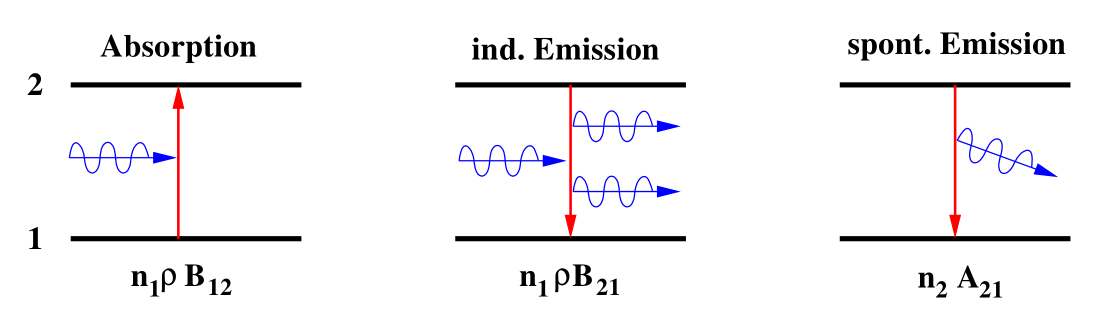
\includegraphics[width = \textwidth]{Pics/EmAb.png}
  \caption{Emission und Absorption. \cite{anleitung}}
  \label{fig:Emission}
\end{figure}

Die Wahrscheinlichkeit, mit der die verschiedenen Vorgänge zwischen zwei Niveaus
auftreten, wird über die Einstein-Koeffizienten $B$ und $A$ bestimmt. Die Anzahl der
spontanen Emissionen pro Zeiteinheit lässt sich wie folgt berechnen, wobei
$A\ua{21}$ die Übergangswahrscheinlichkeit von Niveau $W\ua{2}$ in $W\ua{1}$ darstellt:

\begin{equation}
  n\ua{spon} = N\ua{2}A\ua{21}.
  \label{eqn:Nspon}
\end{equation}

Die Anzahl induzierter Emissionen pro Zeiteinheit ist mit $N\ua{2}$ über den
Einstein-Koeffizienten $B\ua{21}$ sowie dem Strahlungsfeld $\rho$ verbunden:

\begin{equation}
  n\ua{ind} = N\ua{2}B\ua{21}\rho.
  \label{eqn:Nind}
\end{equation}

Durch eine ähnliche Relation lässt sich auch die Anzahl absorbierter Quanten pro
Zeiteinheit bestimmen:

\begin{equation}
  n\ua{abs} = N\ua{1}B\ua{12}\rho.
  \label{eqn:Nabs}
\end{equation}

Unter der Annahme, dass beide Niveaus nicht entartet
sind ($g\ua{1}=g\ua{2}$), gilt $B\ua{12} = B\ua{21}$. Somit lässt sich
$A\ua{21}$ bestimmen, so dass sich die folgende Abhängigkeit ergibt:

\begin{equation}
  A\ua{21} = \frac{8\pi h}{c^3}B\ua{12}\nu^3.
  \label{eqn:A21}
\end{equation}

Im thermischen Gleichgewicht überwiegt dabei gemäß der Maxwell-Boltzmann-Verteilung
die Besetzung des Grundzustandes. Für die zum Lasern benötigte dauerhafte Verstärkung
des Strahlungsfeldes muss die induzierte Emission deutlich häufiger auftreten als
die spontane Emission. Dafür ist eine höhere Besetzung des angeregten Zustandes
nötig, welche auch als Besetzungsinversion bezeichnet wird. Diese wird durch das
optische Pumpen realisiert.

Die Besetzungsinversion ist allerdings in einem reinen 2-Niveau-System wie es hier
verwendet wurde nicht realisierbar. Dies ergibt sich relativ schnell aus Gleichung
\eqref{eqn:NRelation}. Liegen nicht entarteten Zuständen vor, kann lediglich
die Temperatur als Parameter beeinflusst werden. Selbst beim Limes T $\rightarrow$ $\infty$
kann lediglich ein Verhältniss von 50:50 erreicht werden. Zudem kann es auch damit
erklärt werden, dass bei einem Zwei-Nievau-System irgendwann die Wahrscheinlichkeit
für die induzierte Emission genauso hoch ist wie die für die Absorption, genau dann
wenn $n\ua{1}$ = $n\ua{2}$ gilt (siehe \eqref{eqn:Nind} und \eqref{eqn:Nabs}).
Berücksichtigt man anschließend auch noch die spontane Emission, so lässt sich
eine Gleichbesetzung gar nicht erzeugen und es gilt immer $n\ua{1}$ > $n\ua{2}$


\subsection{Besetzungsinversion beim HeNe-Laser}

Bei dem $\ce{HeNe}$-Laser handelt es sich um ein einen Gaslaser mit einem Helium-Neon Verhältnis
von 5 zu 1 bei einem Druck von ca. 133 Pascal. Die Besetzungsinversion wird über eine
elektrische Entladung erzeugt, wobei sie nicht direkt beim Lasermedium Neon erzeugt wird.
Stattdessen wird das Pumpgas Helium vom Grundzustand in einen angeregten, metastabilen
Zustand gehoben.
Da die Energien der $2^1S\ua{0}$ und $2^3S\ua{1}$ Niveaus des Heliums
ungefähr den Energien der $3s$ und $2s$ Niveaus des Neons enstprechen, kann dieses
durch Stöße 2.Art in die beiden angeregten Zustände gehoben werden. Das Helium geht dabei
wieder in den Grundzustand über und kann anschließend erneut angeregt werden.
Somit kann eine Besetzungsinversion beim Neon erzeugt werden (siehe Abbildung \ref{fig:Inversion}).
Die intensivste der auftretenden Spektrallinien ist die rote Linie mit $\lambda$
= 632,8 nm.


\begin{figure}
  \centering
  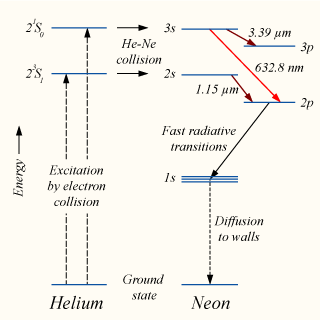
\includegraphics[width = 0.7\textwidth]{Pics/Niveaus.png}
  \caption{Besetzungsinversion beim HeNe-Laser. \cite{Inversion}}
  \label{fig:Inversion}
\end{figure}


\subsection{Resonatoraufbau und Stabilitätsbedingung}
\label{sub:ResStab}

Da die Verstärkung exponentiell mit der Länge des Lasermediums anwächst, wird
ein Resonator verwendet. Dieser besteht im Grunde aus zwei Teilspiegeln,
wovon einer teilreflektierend und einer totalreflektierend ist, sowie dem Lasermedium
(siehe Abbildung \ref{fig:Resonator}). Durch die beiden Spiegel durchläuft der Strahl
mehrfach das Medium, wobei immer ein Teil an dem teildurchlässigem Spiegeln
ausgekoppelt wird. Für den Resonator können dabei verschiedene Spiegel benutzt werden.
Allerdings müssen für einen selbstanregenden Oszillator die Verluste möglichst gering
gehalten werden, was besonders durch konkave Spiegel realisiert werden kann.
Ein Beispiel dafür ist der konfokale Resonator, bei dem die Spiegelbrennpunkte zusammenfallen.
Sind die enstehenden Verluste kleiner als die Verstärkung, so wird von einem
optisch stabilen selbsterregenden Oszillator gesprochen.

\begin{figure}
  \centering
  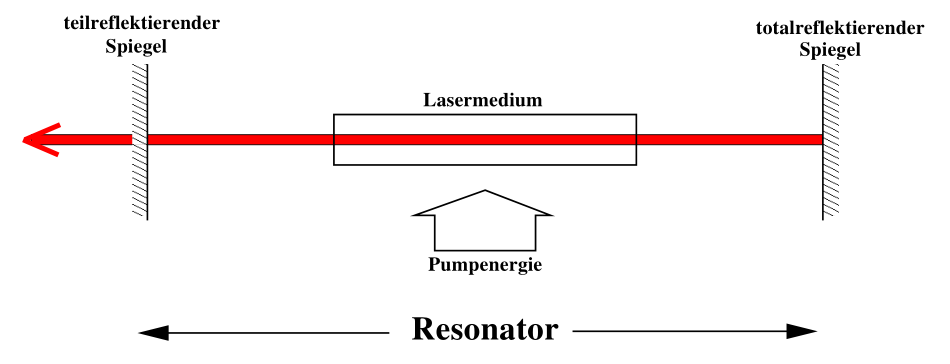
\includegraphics[width = 0.8\textwidth]{Pics/Resonator.png}
  \caption{Schematischer Aufbau eines Resonators. \cite{anleitung}}
  \label{fig:Resonator}
\end{figure}

Die Stabilität eines Resonators kann dabei auch quantitativ durch die Stabilitätsbedingung
erfasst werden:

\begin{equation}
  0 \leq g\ua{1}\cdot g\ua{2} \leq 1.
\end{equation}

Der Resonatorparameter $g\ua{i} = 1 - \frac{L}{r\ua{i}}$ wird dabei durch die
Resonatorlänge $L$ und den Krümmungsradius $r$ bestimmt. Für den $\ce{HeNe}$-Laser wird dabei
ein fester konkaver Spiegel mit $r\ua{1} = 1400 \, mm$ verwendet, der wahlweise
durch einen planparallelen Spiegel ($r\ua{2} = \infty$) oder einen weiteren konkaven
Spiegel ($r\ua{2} = r\ua{1}$) ergänzt wird. Der Verlauf des Faktors $g\ua{1}\cdot g\ua{2}$
ist in Abbildung \ref{fig:g1g2}.

\begin{figure}
  \centering
  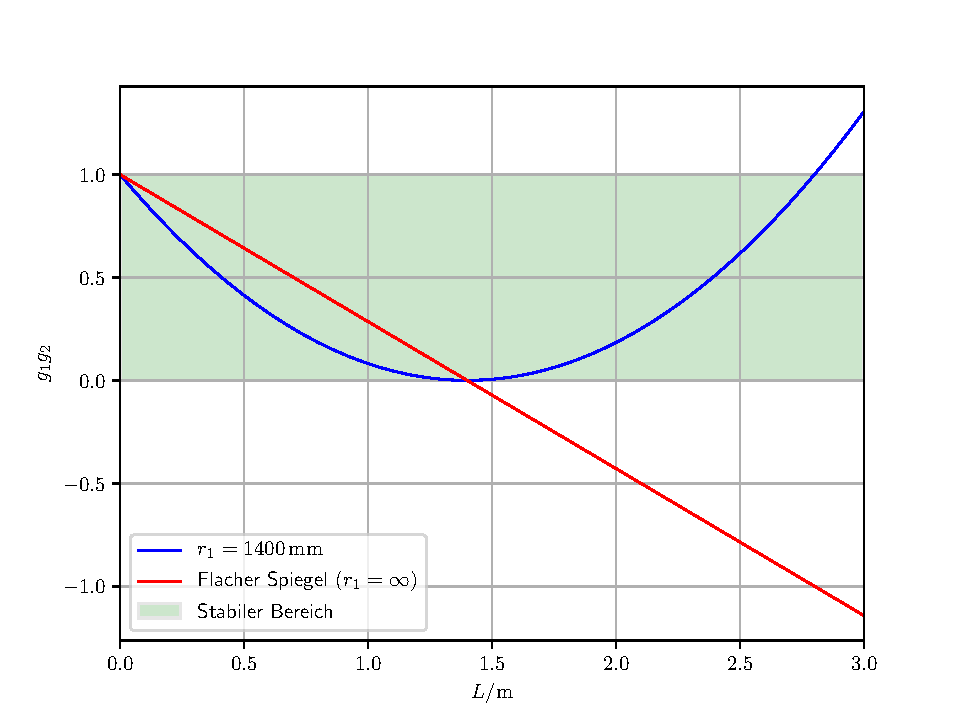
\includegraphics[width = \textwidth]{Pics/g_1_g_2.pdf}
  \caption{Verlauf des Stabilitätsparameters. \cite{StevenStefan}}
  \label{fig:g1g2}
\end{figure}

\subsection{Elektromagnetische Moden des Lasers}

Im Allgemeinen ist die Resonatorlänge deutlich größer als die Wellenlänge $\lambda$
des emittierten Lichtes. Somit können mehrere Moden auftauchen. Die Anzahl q der
Wellenlängen im Resonator wird als longitudinale Mode bezeichnet. Aufgrund von
Unebenheiten der Spiegeloberflächen treten zusätzlich auch transversale Moden auf,
die im folgenden als $TEM\ua{lp}$ (transverse electromagnetic mode) bezeichnet werden.
Bei l handelt es sich dabei um die Anzahl der auftretenden Knoten in x-Richtung und bei p
dementsprechend um die Anzahl der Knoten in y-Richtung. Da höhere Moden auch
höhere Verluste erzeugen, sind im Resonator nur wenige transversale Moden stabil
und werden verstärkt.

Die Mode mit der höchsten Symmetrie und den niedrigsten Verlusten ist die $TEM\ua{00}$-Mode,
welche keine Nullstelle in transversaler Richtung besitzt. Die Insitätverteilung
folgt dabei einer Gaußverteilung:

\begin{equation}
  I(r) = I\ua{0} \exp{(-\frac{2r^2}{\omega^2})}.
\end{equation}

$I\ua{0}$ ist dabei die Maximalintensität, $r$ der Abstand zur optische Achse und 2$\omega$
der Strahldurchmesser. Der Strahlradius $\omega$ lässt sich über den Abstand z zur
minimalen Strahltaille $\omega\ua{0}$ definieren:

\begin{equation}
  \omega(z) = \omega\ua{0} \sqrt{1 + \left( \frac{\theta z}{\omega\ua{0}} \right)^2}.
\end{equation}

Bei $\theta=(\lambda/\pi)\omega\ua{0}$ handelt es sich um die Strahldivergenz.

Neben der Grundmode wird zudem die $TEM\ua{01}$ untersucht. Diese ist allerdings
viel schwächer als die Grundmode. Deswegen wird mittels einer Modenblende die
$TEM\ua{00}$-Mode unterdrückt. Für die $TEM\ua{01}$-Mode ergibt sich dann eine
doppelte Gauß-Funktion als Intensitätsverteilung:

\begin{equation}
  I(r) = I\ua{0}\cdot(\exp{(-\frac{2(r-r\ua{1})^2}{\omega^2})} + \exp{(-\frac{2(r+r\ua{1})^2}{\omega^2})}).
\end{equation}

\subsection{Brewster-Fenster}
\label{sub:Brewster}

Zum Auskoppeln des Strahls aus der HeNe-Röhre wird ein Brewster-Fenster verwendet.
Im Gegensatz zu Abbildung \ref{fig:Brewster} befindet bei diesem Versuch auf beiden
Seiten der HeNe-Röhre nur eine Platte.
Bei dem Winkel zwischen Strahl und Platte handelt es sich um den Brewster-Winkel,
bei dem ausschließlich das zur Einfallsebenen senkrecht polarisierte Licht
reflektiert wird. Das parallel polarisierte Licht kann jedoch nahezu verlustfrei
in die HeNe-Röhre eintreten bzw. aus der Röhre austreten. Bei zwei senkrechten
Fenstern hingegen wären die Verluste durch Reflektion zu hoch, um einen selbsterregenden
Oszillator zu realisieren.

\begin{figure}
  \centering
  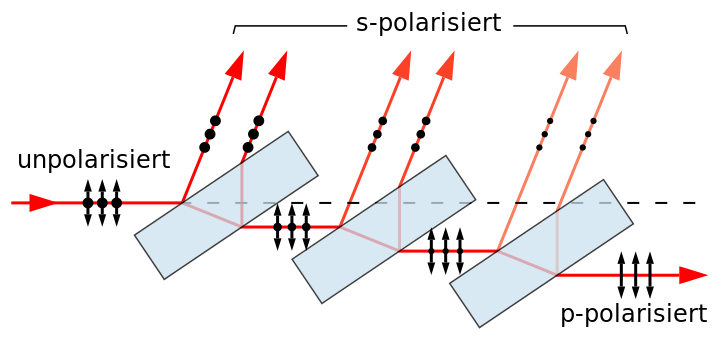
\includegraphics[width = 0.8\textwidth]{Pics/Brewster.png}
  \caption{Aufbau eines Brewster-Fensters. \cite{Brewster}}
  \label{fig:Brewster}
\end{figure}

\section{Aufbau und Durchführung}

Der komplette Versuch wird auf einer optischen Schiene aufgebaut. Der Justierlaser
($\lambda$ = 532 nm, $P\ua{max}$ = 1 mW) wird mit einer reduzierten Laserleistung
von $P\ua{red}$ = 0,2 mW betrieben. Der Strahl des Justierlasers geht durch eine
Blende, auf deren Rückseite sich ein Fadenkreuz zur Justierung der Spiegel befindet.
Neben dem Justierlaser befindet sich der
eigentliche Aufbau des $\ce{HeNe}$-Lasers, bestehend aus zwei hochreflektierenden Spiegeln
und einem Laserrohr mit dem Helium-Neon-Gemisch, welche zusammen den Laserresonator
bilden. Das Laserrohr hat eine Länge von l = 408 mm und einen Durchmesser
von $d\ua{HeNe}$ = 1,1 mm. In dem Laserrohr befinden sich die Elektroden, mit denen
das Helium über elektrische Entladungen angeregt wird, um über Stöße 2. Art
die Besetzungsinversion im Neon zu
erzeugen. Am beiden Enden des Laserrohrs befindet sich
ein Brewster-Fenster (siehe Abschnitt \ref{sub:Brewster}).
Die zur Verfügung stehenden Spiegel haben alle
einen Durchmesser von $d\ua{Spiegel}$ = 12,7 mm.

Zum Vermessen der verschiedenen Eigenschaften stehen entsprechende Komponenten
neben der Apparatur bereit, welche bei der entsprechenden Messung auf die optische
Schiene montiert werden können. Dazu gehören eine Photodiode, ein Polarisator, ein
Wolfram-Draht und ein Gitter. Die Komponenten sind alle an Halterungen angebracht,
welche zum Teil mittels Mikrometerschrauben im Strahlengang verschoben werden
können.

\begin{figure}
  \centering
  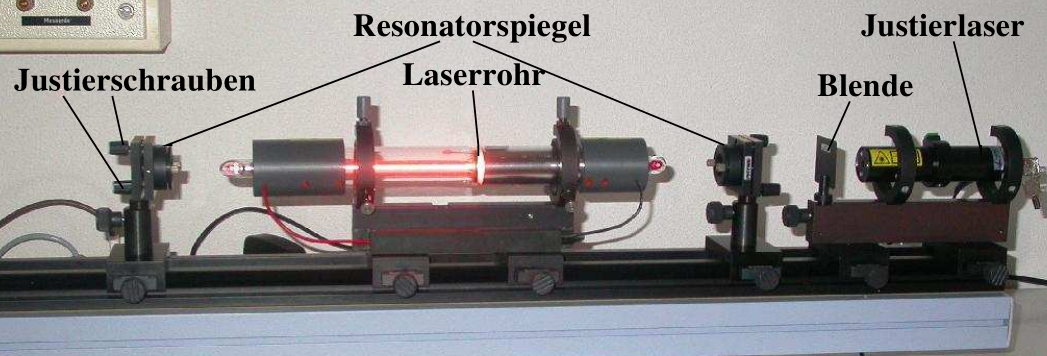
\includegraphics[width = \textwidth]{Pics/Aufbau.png}
  \caption{Aufbau des $\ce{HeNe}$-Lasers. \cite{anleitung}}
  \label{fig:HENE}
\end{figure}

Zu Beginn des Versuches müssen zuerst mittels des Justierlasers die beiden Spiegel
justiert werden. Dafür wird erst der hintere Spiegel (konkav) in den Strahlengang gestellt
und so justiert, dass der reflektierte Strahl genau auf die Mitte des Fadenkreuzes
fällt. Danach wird der vordere Spiegel (konkav) in den Strahlengang gestellt und die selbe
Justage wiederholt. Anschließend wird das Laserrohr mit einem Betriebsstrom von
$I$ = 6,5 mA auf der optischen Schiene befestigt. Die beiden Resonatorspiegel
werden mithilfe der Justierschrauben noch nachjustiert, bis das Gasgemisch lasert
und die rote Linie deutlich erkennbar ist.

Als erstes wird mit dem Polarisationsfilter die Intensität in abhängigkeit von
der Polarisationsrichtung gemessen. Dafür wird der Filter in 10° Schritten gedreht
und jedesmal mithilfe der Photodiode die Intensität gemessen.
Danach wird zuerst die $TEM\ua{00}$-Mode vermessen. Dafür wird der Strahl mittels
einer Linse aufgefächert, sodass mit der Photodiode die Intensität vermessen werden kann.
Die Photodiode wird dabei von einer Kante des Strahls in 1 mm Schritten bis zur
anderen Kante der Strahls gefahren.
Anschließend wird der Wolfram-Draht innerhalb des Resonators zwischen die HeNe-Röhre
und den auskoppelnden Spiegel in den Strahlengang
gebracht, um die $TEM\ua{01}$-Mode
sichtbar zu mache. Der "Wellenbauch" bzw. das Intensitätsmaximum der $TEM\ua{00}$-Mode
befindet sich in der Mitte des Strahles, weswegen dort der Wolfram-Draht platziert
wird. Anschließend wird wie schon bei der vorherigen Mode beschrieben die Intensität
des Strahles vermessen, ebenfalls in 1 mm Schritten.
Danach werden mithilfe eines Gitters die Beugunsmaxima verschiedener
Ordnungen auf einem Schirm sichtbar gemacht und die jeweiligen Abstände zum
Maximum 0. Ordnung mittels eines Maßbandes vermessen.

Zum Schluss wird dann die Stabilitätsbedingung für den Laser überprüft. Dafür wird
der Abstand zwischen den beiden Spiegeln in 10 cm Schritten vergrößert und jedes
mal nach Einjustieren die Intensität mittels der Photodiode vermessen.

Anschließend wird der konkave Spiegel zwischen Justierlaser und Laserrohr
ausgetauscht und ein planparalleler
Spiegel eingesetz. Dafür muss die Apparatur auch noch einmal komplett neu
justiert werden. Anschließend wird die Stabilitätsbedingung im selben
Muster wie bei dem vorherigem Aufbau durchgeführt.
